\documentclass[UTF8]{ctexart}
\usepackage{algpseudocode}
\usepackage{algorithm}
\usepackage{amsmath}
\usepackage{subcaption}
\usepackage{graphicx}
\usepackage[bottom=4em]{geometry}
\usepackage{lmodern}
\usepackage{listings}
\usepackage{xcolor}

\ctexset{ section = { format={\Large \bfseries } } }

\pagestyle{empty}

\begin{document}

\section*{Task 1:Loop Mesh Subdivision}

在每次迭代中,对于原先存在的顶点和边分别计算其新位置,最后把每个三角形分为四个。由于提供的 DCEL 没有赋予边编号,所以我使用了一个 map 来记录编号。

\begin{figure}[h]
    \begin{subfigure}[b]{0.48\textwidth}
        \centering
        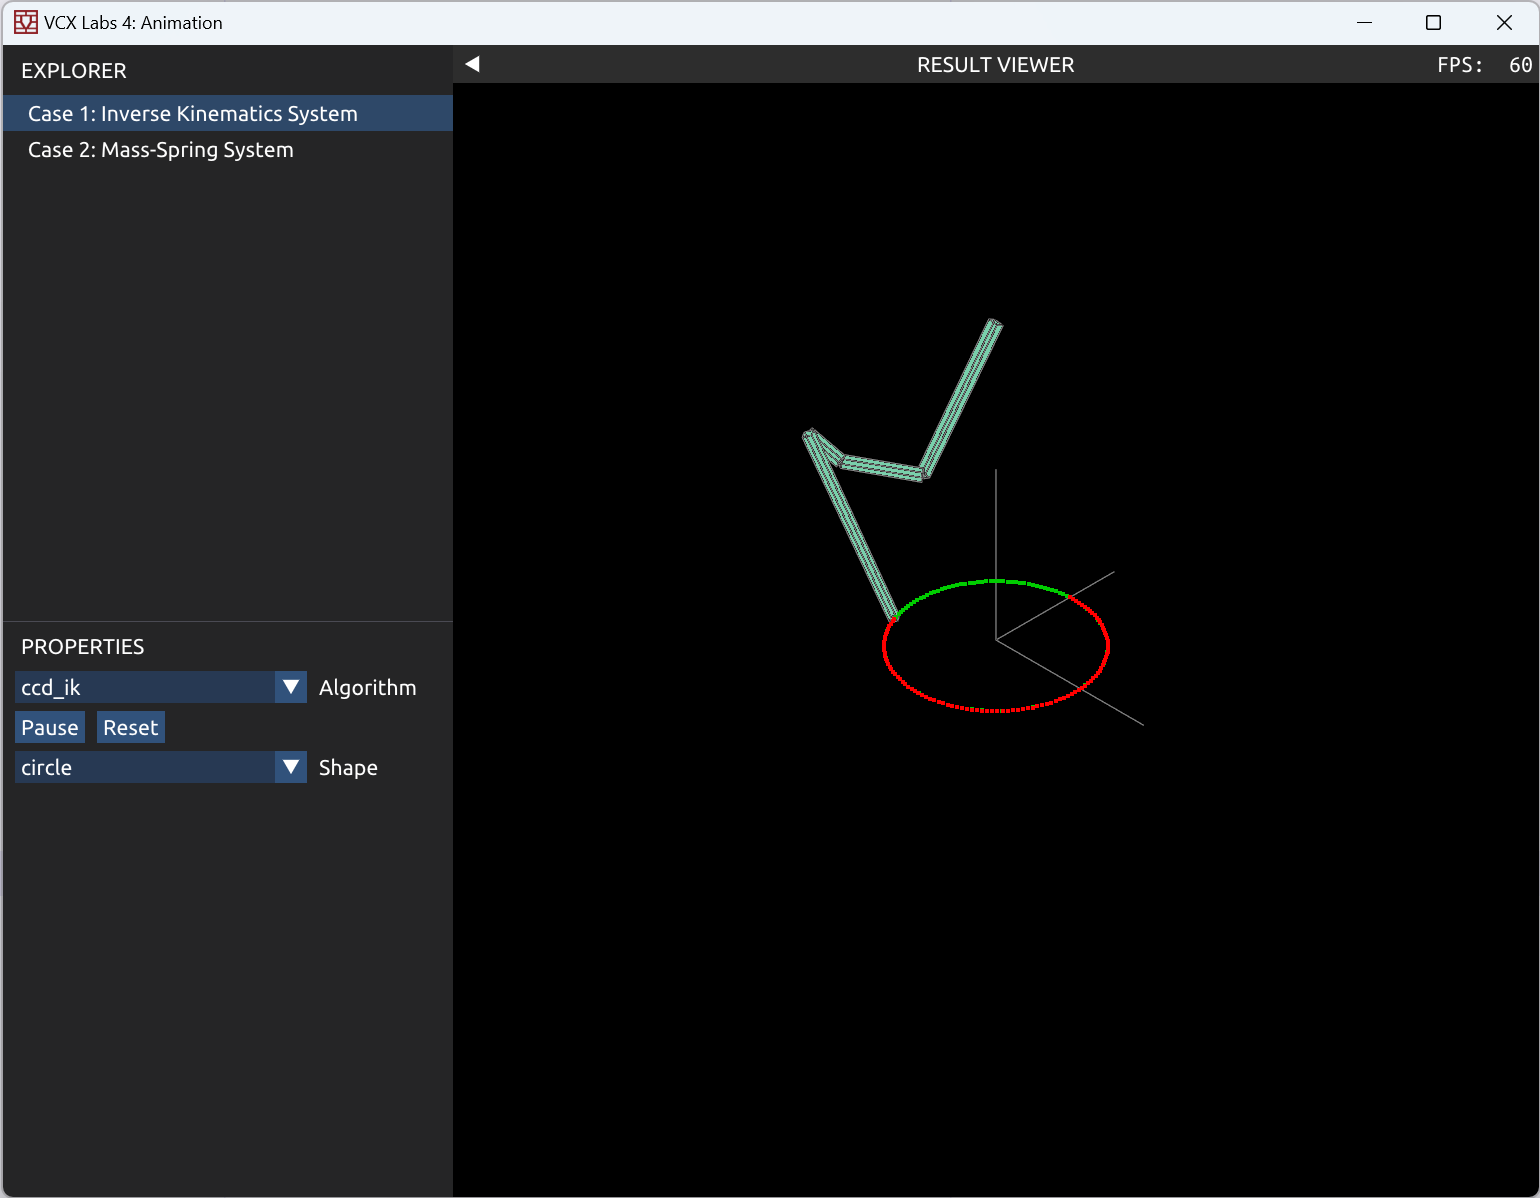
\includegraphics[height=0.3\textheight]{images/1-1.png}
        \caption{block.obj 迭代一次结果}
    \end{subfigure}
    \hfill
    \begin{subfigure}[b]{0.48\textwidth}
        \centering
        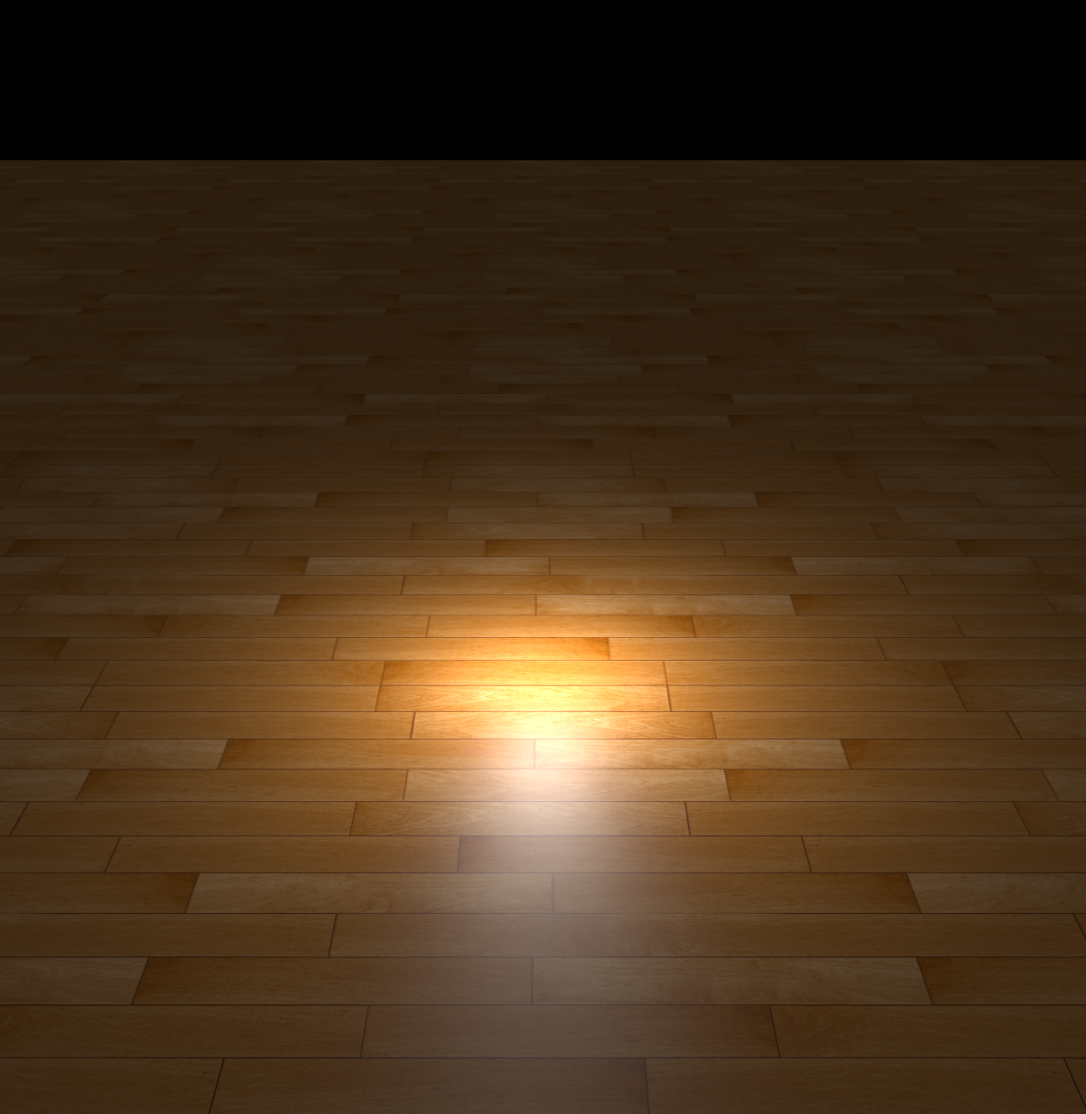
\includegraphics[height=0.3\textheight]{images/1-2.png}
        \caption{dinosaur.obj 迭代三次结果}
    \end{subfigure}
\end{figure}

\section*{Task 2:Spring-Mass Mesh Parameterization}

从任意一个边界点出发,按照任意顺序(顺时针或逆时针)不断寻找下一个边界点直到回到起点。把所有边界点按顺序映射到纹理平面上以 $(0.5, 0.5)$ 为圆心,$0.5$ 为半径的圆周上的等分点。最后使用 Jacobi 迭代求解内部点的位置。

\begin{figure}[h]
    \begin{subfigure}[b]{0.32\textwidth}
        \centering
        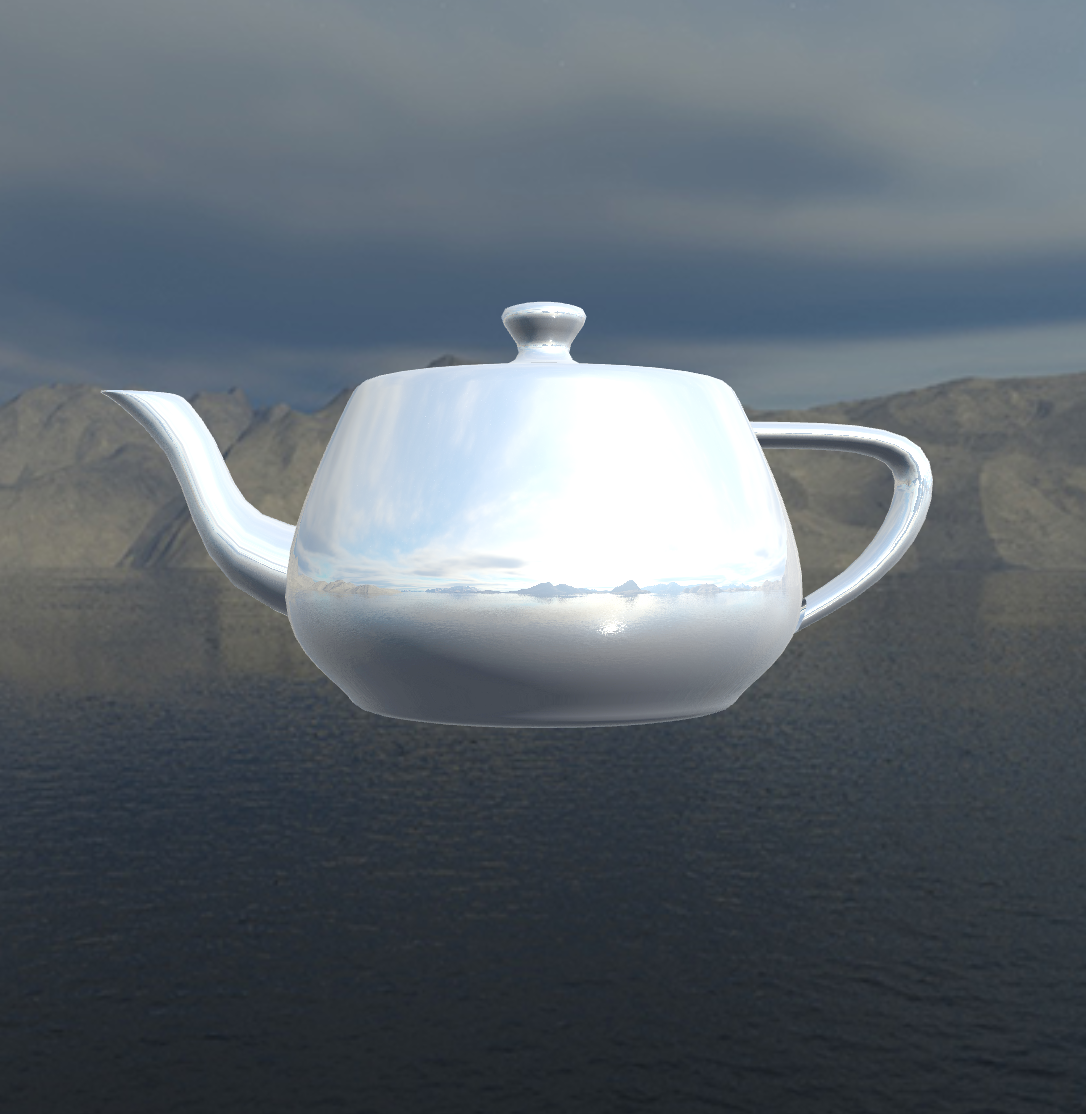
\includegraphics[height=0.3\textheight]{images/2-1.png}
        \caption{迭代 $50$ 次}
    \end{subfigure}
    \hfill
    \begin{subfigure}[b]{0.32\textwidth}
        \centering
        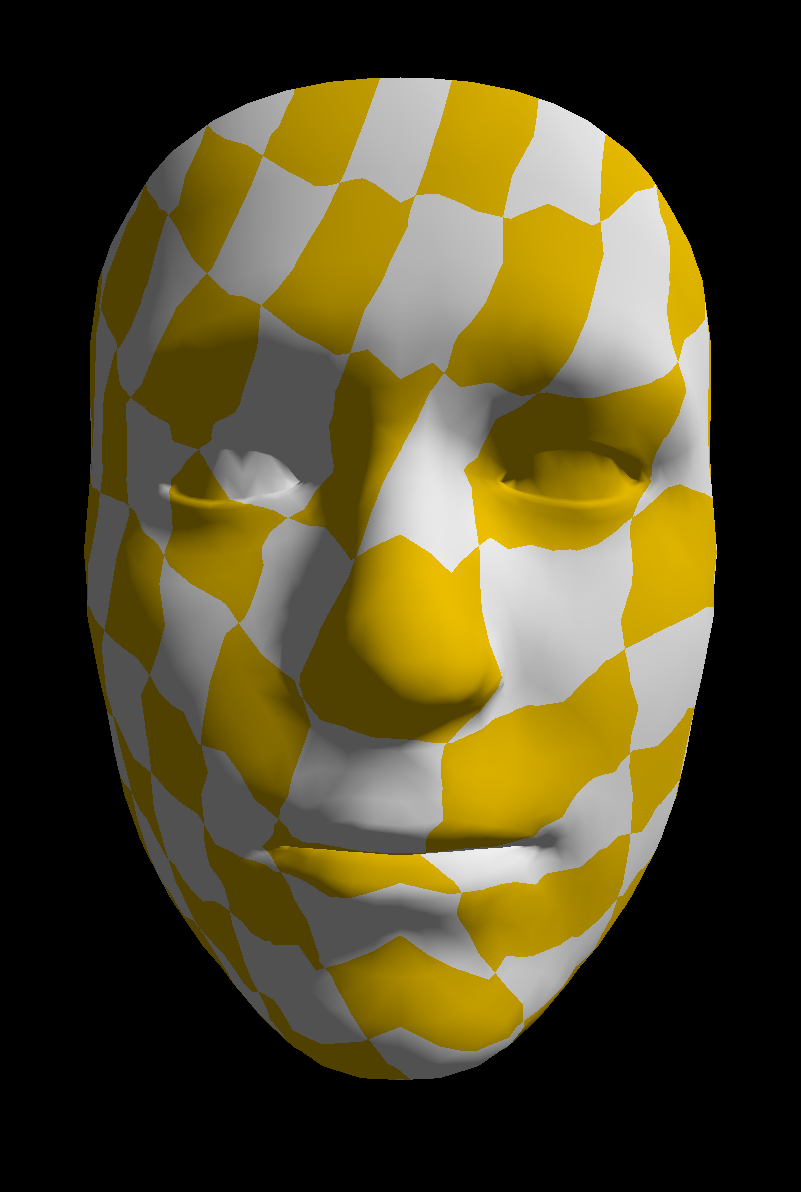
\includegraphics[height=0.3\textheight]{images/2-2.png}
        \caption{迭代 $300$ 次}
    \end{subfigure}
    \hfill
    \begin{subfigure}[b]{0.32\textwidth}
        \centering
        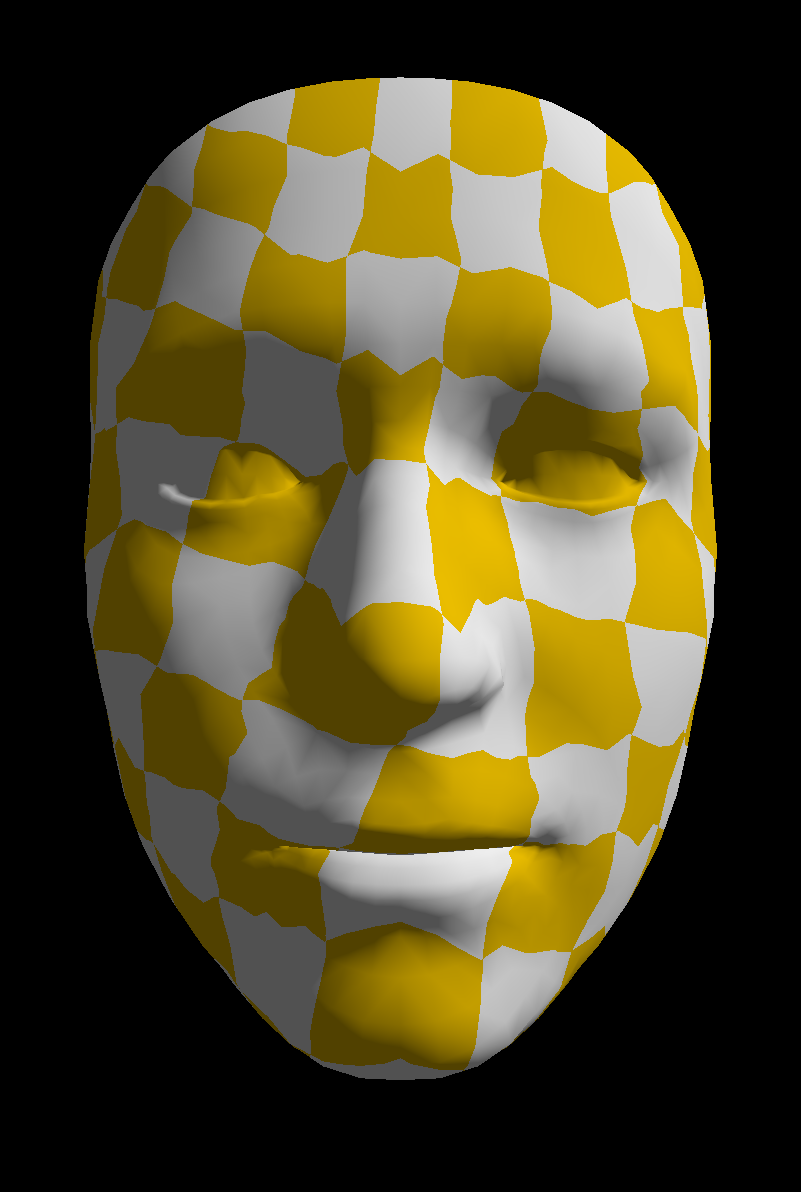
\includegraphics[height=0.3\textheight]{images/2-3.png}
        \caption{迭代 $1000$ 次}
    \end{subfigure}
\end{figure}

\section*{Task 3:Mesh Simplification}

按照论文中的方法,对每个初始顶点计算矩阵 $Q$。然后枚举所有直接相邻或者距离不超过阈值的顶点对,计算合并的最小代价。最后不断选择代价最小的顶点对进行合并,更新相应信息,直到剩余顶点比例不超过给定值。代价的计算过程与论文中的方法完全相同。

\begin{figure}[h]
    \begin{subfigure}[b]{0.48\textwidth}
        \centering
        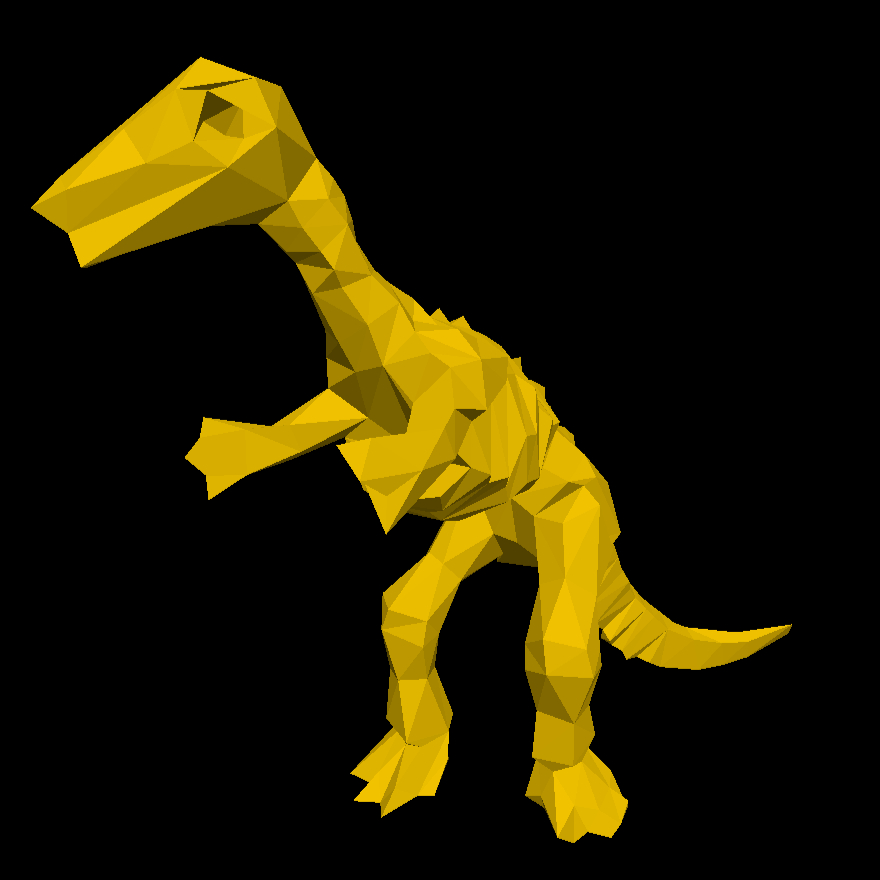
\includegraphics[height=0.3\textheight]{images/3-1.png}
        \caption{dinosaur.obj 最高等级化简结果}
    \end{subfigure}
    \hfill
    \begin{subfigure}[b]{0.48\textwidth}
        \centering
        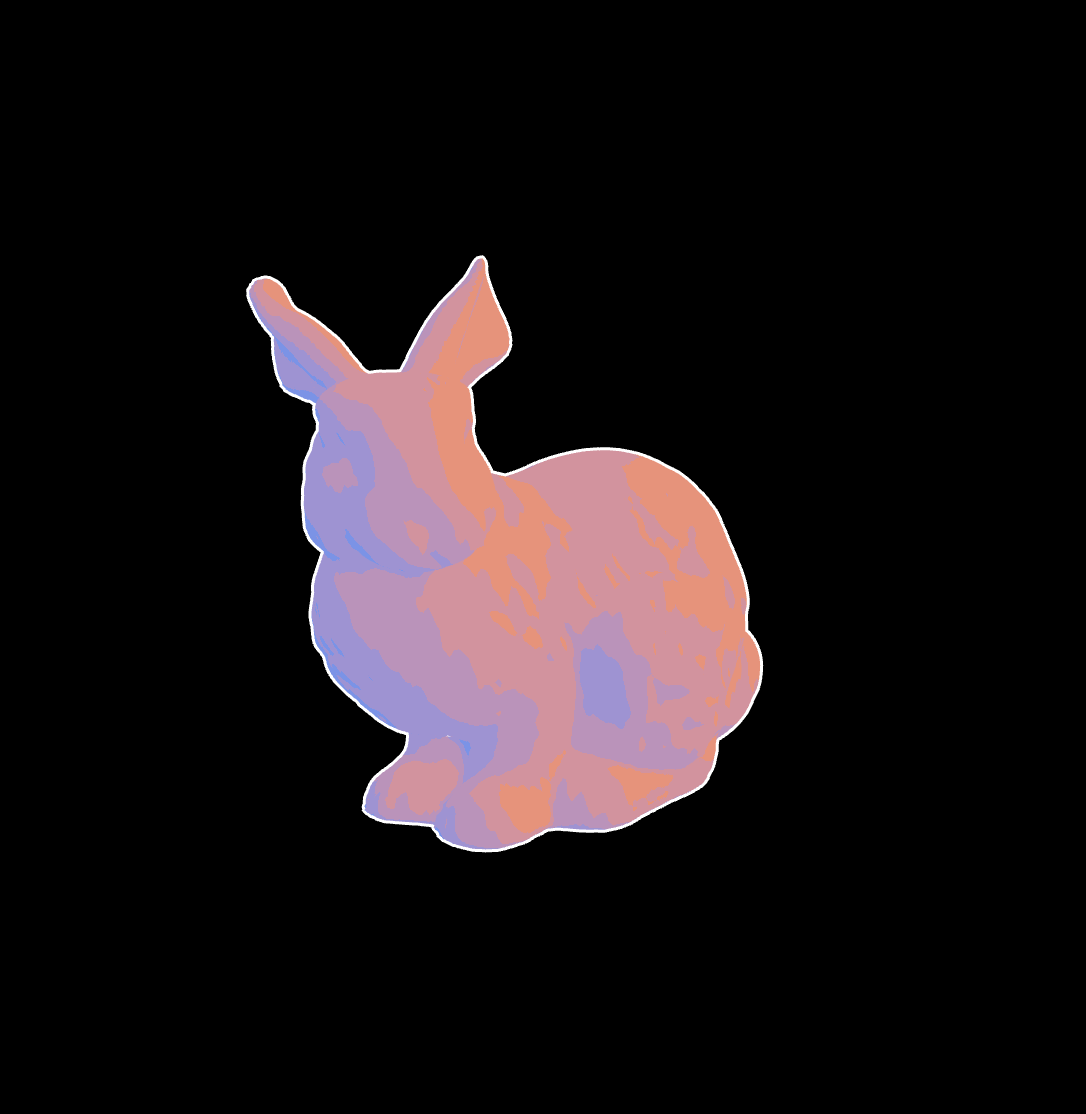
\includegraphics[height=0.3\textheight]{images/3-2.png}
        \caption{arma.obj 最高等级化简结果}
    \end{subfigure}
\end{figure}

\section*{Task 4:Mesh Smoothing}

按照给定的方法逐步计算。

\begin{figure}[h]
    \begin{subfigure}[b]{0.48\textwidth}
        \centering
        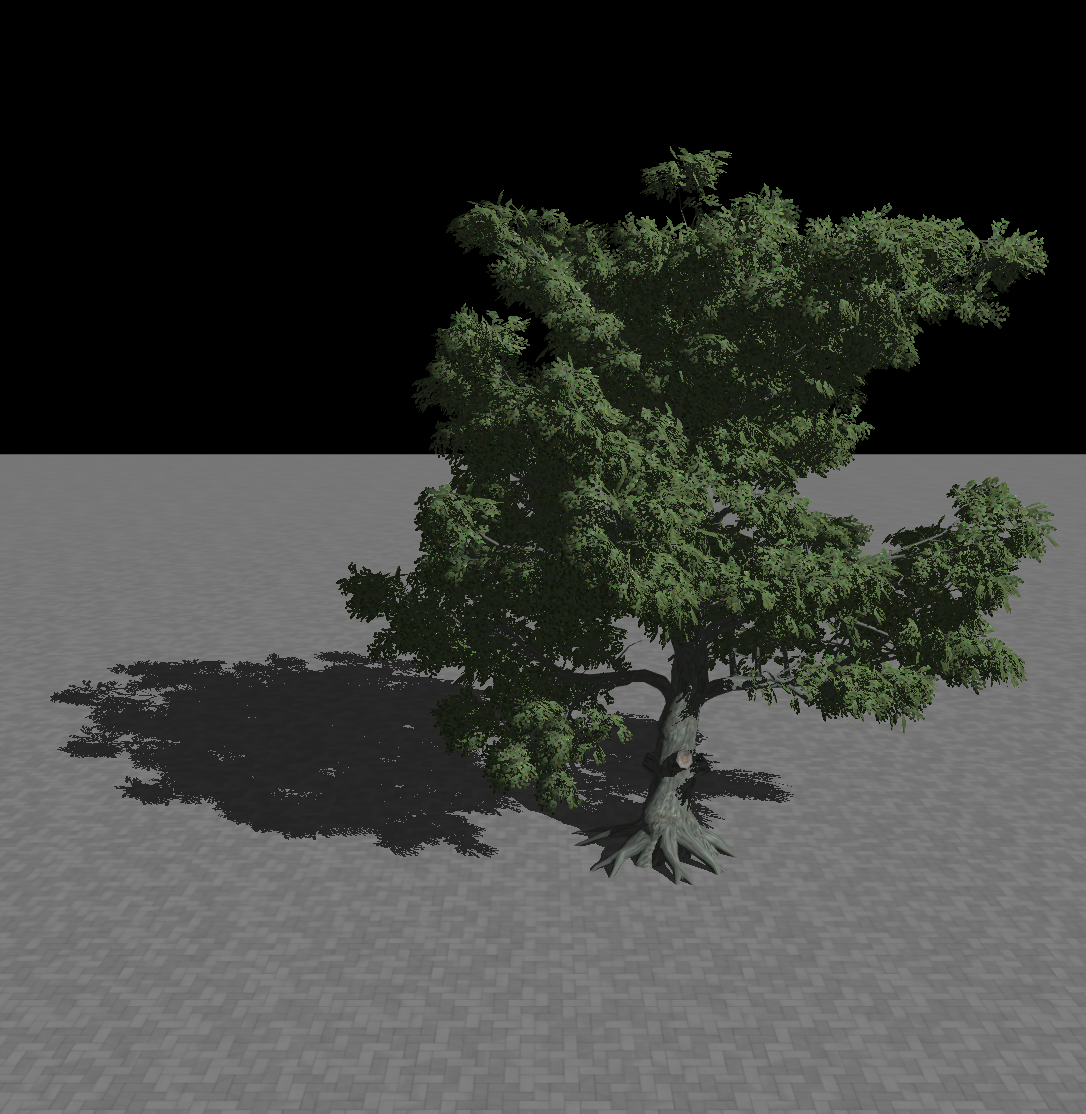
\includegraphics[height=0.3\textheight]{images/4-1.png}
        \caption{block.obj 使用 Uniform Weight 和 Smoothness 0.9 迭代 5 次}
    \end{subfigure}
    \hfill
    \begin{subfigure}[b]{0.48\textwidth}
        \centering
        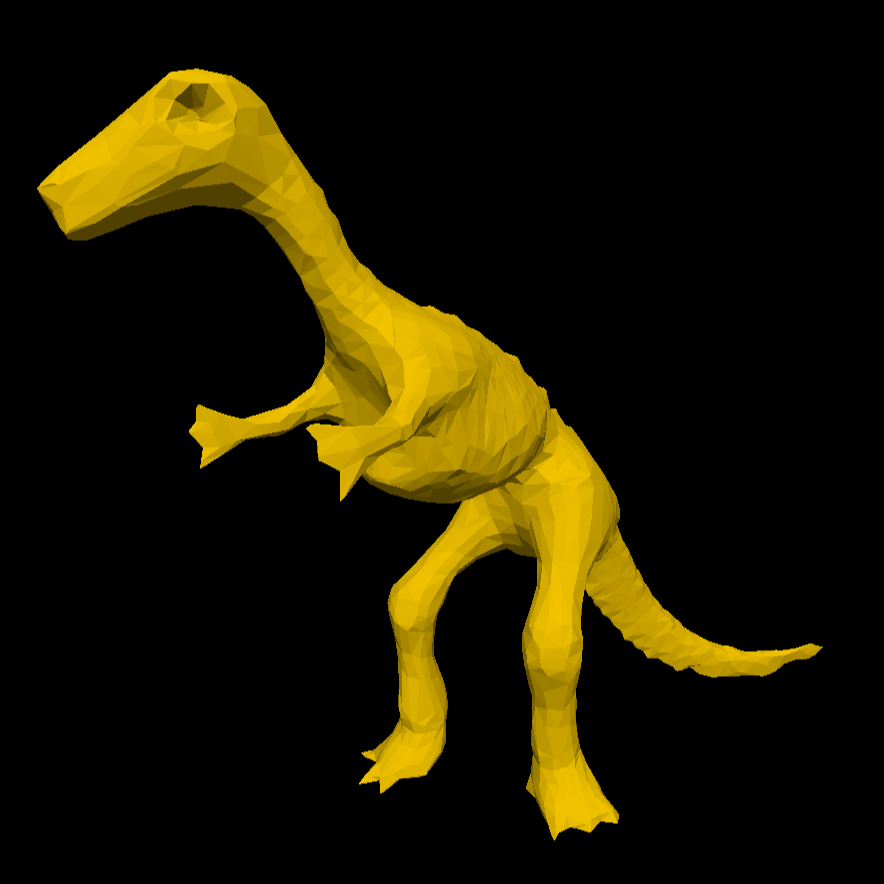
\includegraphics[height=0.3\textheight]{images/4-2.png}
        \caption{dinosaur.obj 使用 Cotangent Weight 和 Smoothness 0.9 迭代 3 次}
    \end{subfigure}
\end{figure}

\section*{Task 5:Marching Cubes}

枚举每个立方体,计算八个顶点中哪些位于内部(距离场的值为负),然后从提供的表格中找出需要添加的三角形。顶点位置的计算使用线性插值。为了维护公共顶点,我使用了 map 来记录编号。


\begin{figure}[h]
    \begin{subfigure}[b]{0.48\textwidth}
        \centering
        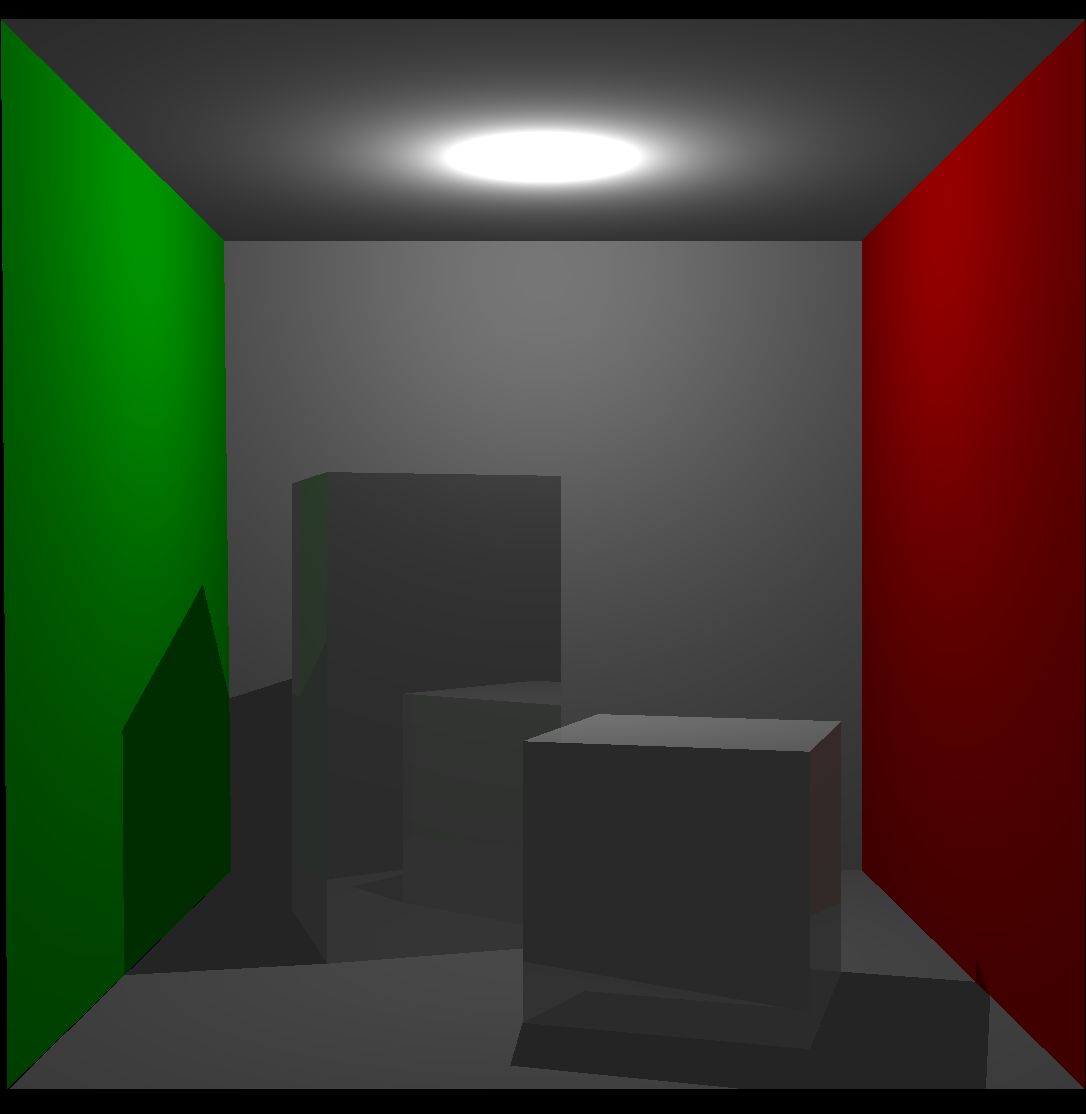
\includegraphics[height=0.3\textheight]{images/5-1.png}
        \caption{Sphere 在 Resolution 为 20 时的结果}
    \end{subfigure}
    \hfill
    \begin{subfigure}[b]{0.48\textwidth}
        \centering
        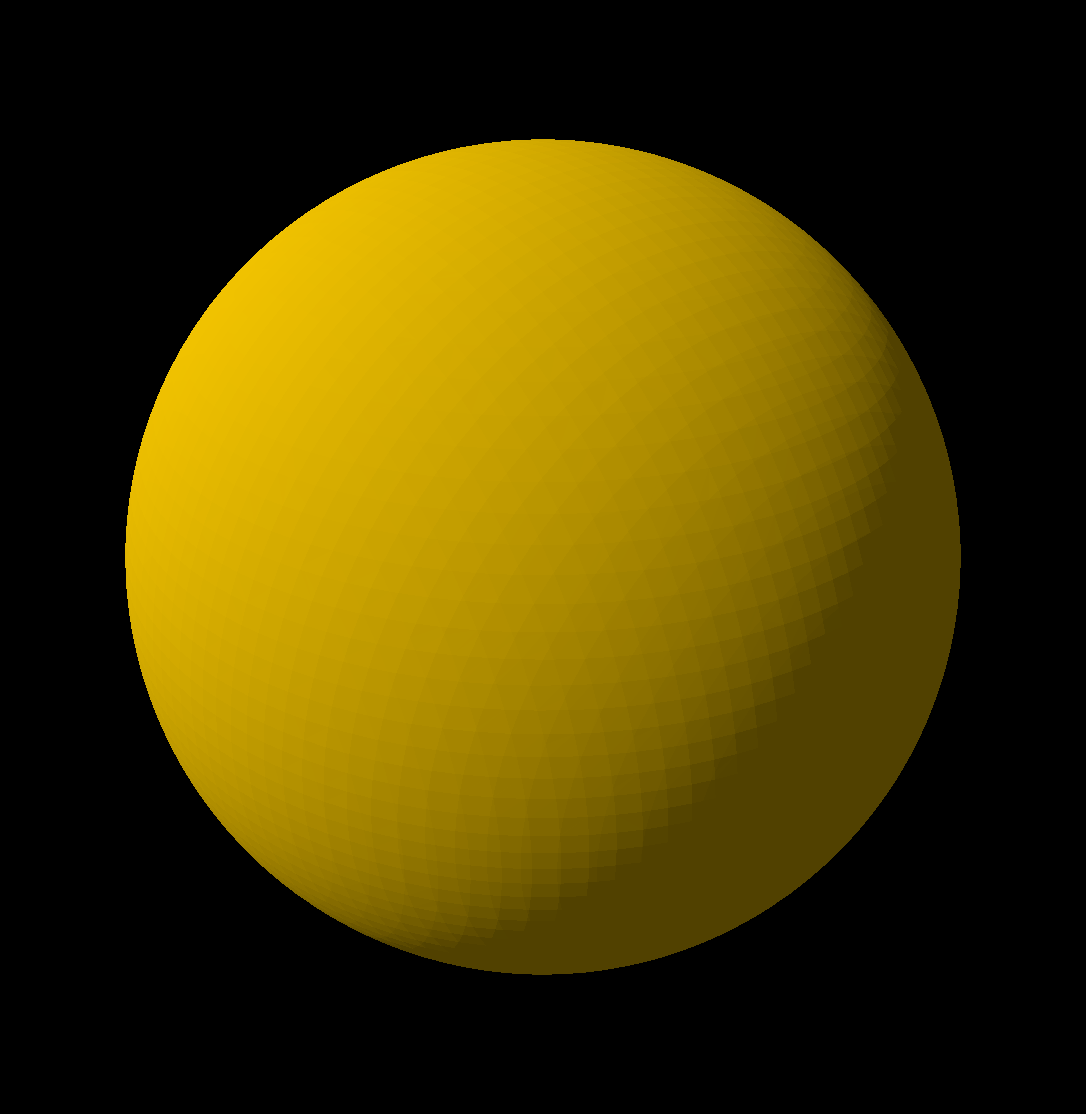
\includegraphics[height=0.3\textheight]{images/5-2.png}
        \caption{Sphere 在 Resolution 为 100 时的结果}
    \end{subfigure}
    \begin{subfigure}[b]{0.48\textwidth}
        \centering
        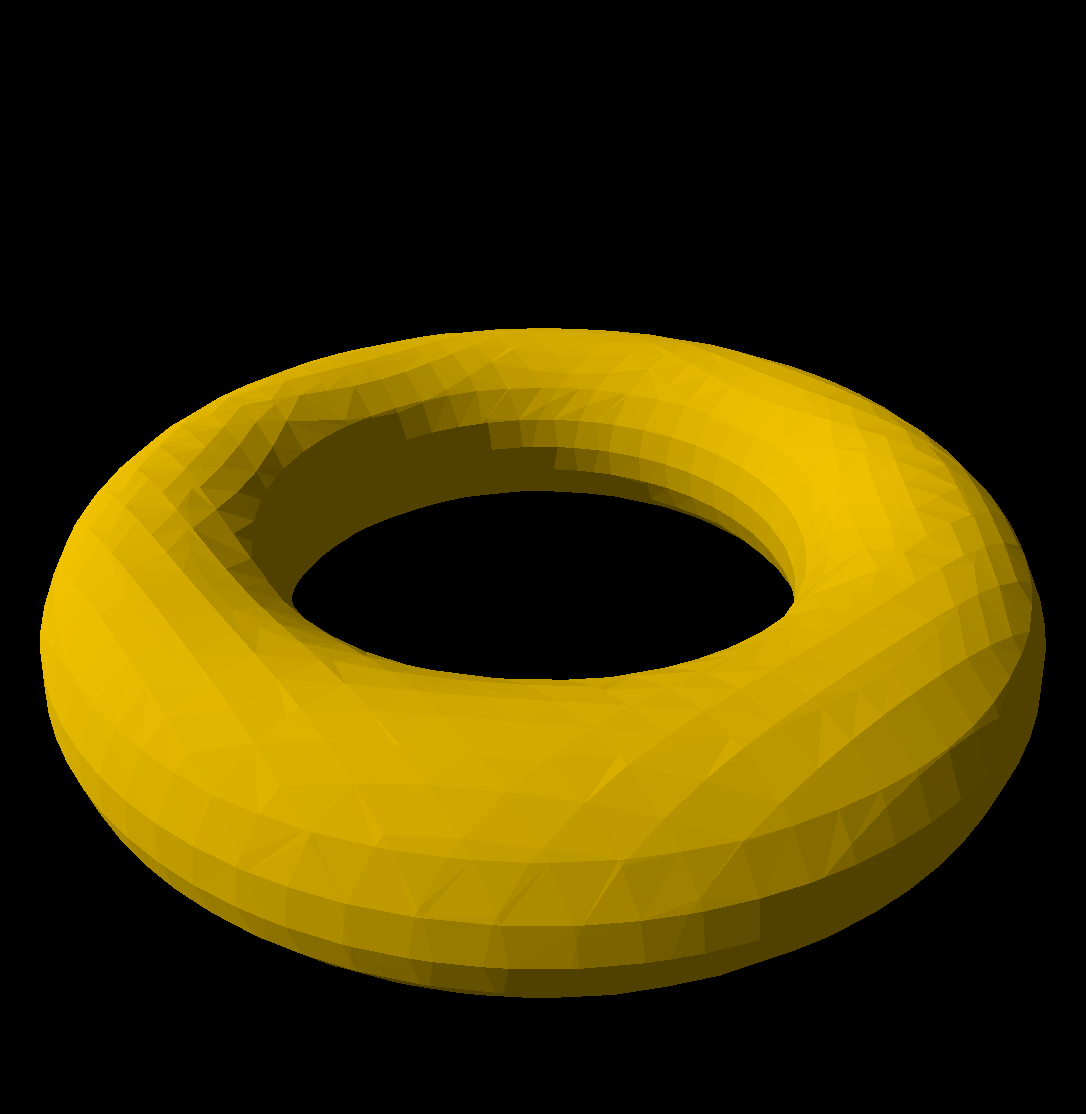
\includegraphics[height=0.3\textheight]{images/5-3.png}
        \caption{Torus 在 Resolution 为 30 时的结果}
    \end{subfigure}
    \hfill
    \begin{subfigure}[b]{0.48\textwidth}
        \centering
        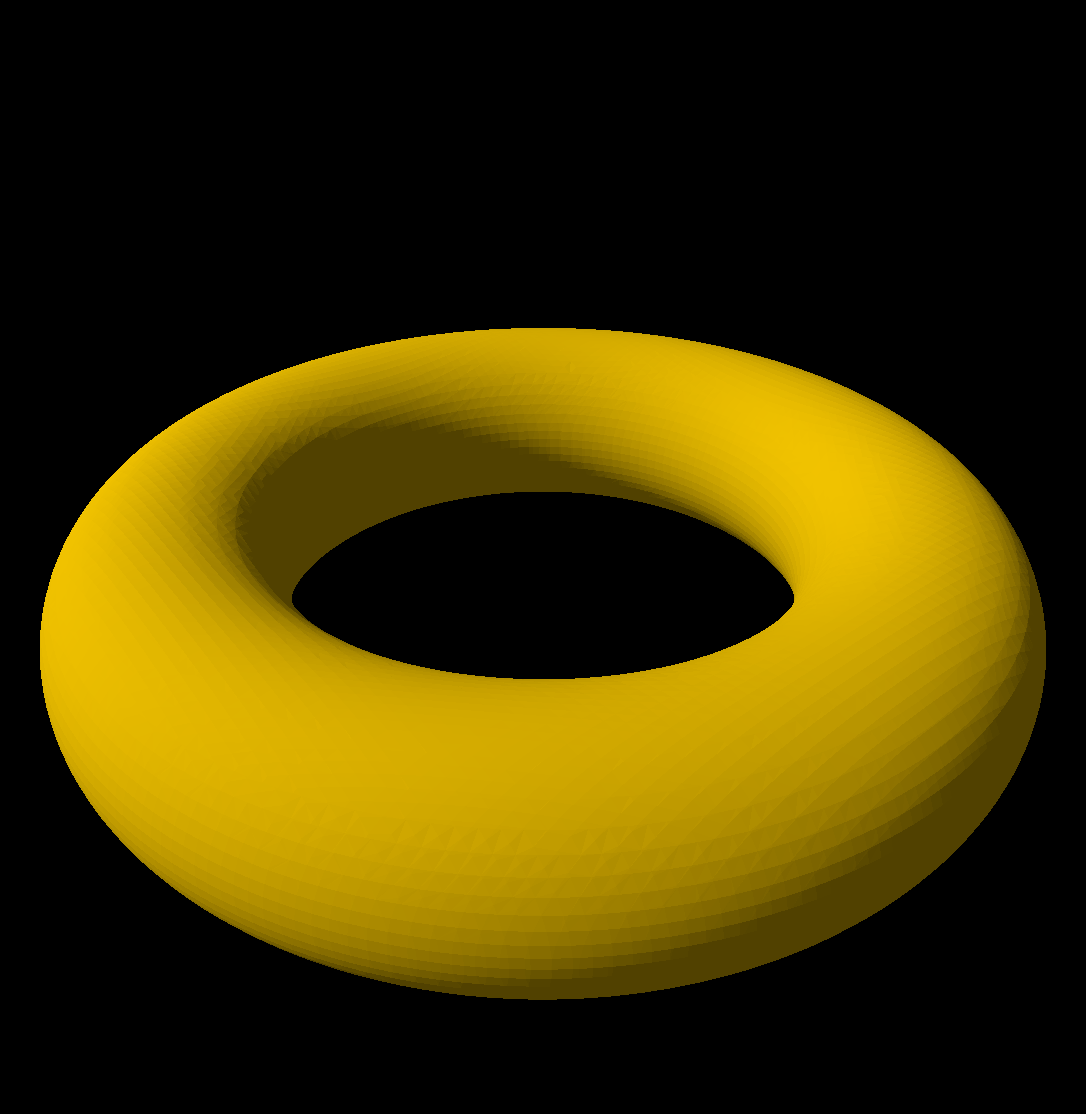
\includegraphics[height=0.3\textheight]{images/5-4.png}
        \caption{Torus 在 Resolution 为 100 时的结果}
    \end{subfigure}
\end{figure}

\end{document}